\section{\K 阻感容元件串联的交流电路}
\Par 如图\ref{fig:串联阻感容}所示,我们考虑这样一个电阻、电感和电容串联的交流电路
\begin{figure}[htbp]
	\centering
	\includegraphics[width=0.65\textwidth]{串联阻感容.pdf}
	\caption{串联阻感容}
	\label{fig:串联阻感容}
\end{figure}

\Par 根据基尔霍夫电压定律我们可以得到
\begin{equation*}
    \dot{U}=\dot{U}_R+\dot{U}_L+\dot{U}_C=\left[ R+\mathrm{j}\left( X_{\mathrm{L}}-X_{\mathrm{C}} \right) \right] \dot{I}
\end{equation*}
其中,我们定义
\begin{equation}
    Z=\frac{\dot{U}}{\dot{I}}=R+\mathrm{j}\left( X_{\mathrm{L}}-X_{\mathrm{C}} \right) 
\end{equation}
为\hl{阻抗},写作$Z$.
\begin{align*}
	Z&=R+\mathrm{j}\left( X_{\mathrm{L}}-X_{\mathrm{C}} \right)\nonumber \\
	&=\sqrt{R^2+\left( X_{\mathrm{L}}-X_{\mathrm{C}} \right) ^2}\cdot \exp \left( \arctan \frac{X_{\mathrm{L}}-X_{\mathrm{C}}}{R} \right)\nonumber \\
	&=\left| Z \right|\mathrm{e}^{\mathrm{j}\varphi}=\left| Z \right|\sin \left( \omega t+\varphi \right) 
\end{align*}
其中
\begin{equation}
    \frac{U}{I}=\sqrt{R^2+\left( X_{\mathrm{L}}-X_{\mathrm{C}} \right) ^2}=\left| Z \right|
\end{equation}
被称作\textbf{阻抗模}.
\begin{equation}
    \varphi =\arctan \left( \frac{X_{\mathrm{L}}-X_{\mathrm{C}}}{R} \right) =\arctan \left( \frac{U_{\mathrm{L}}-U_{\mathrm{C}}}{U_{\mathrm{R}}} \right) 
\end{equation}
被称作\textbf{阻抗角}.阻抗反映了总电压$\dot{U}$与总电流$\dot{I}$之间的大小($\left| Z \right|$)关系和相位($\varphi$)关系,但需要注意的是,它不代表正弦量,因此也不是相量.

\Par 当电路中$X_{\mathrm{L}}-X_{\mathrm{C}}>0$时,电压超前于电流,我们称其为\textbf{感性电路};当电路中$X_{\mathrm{L}}-X_{\mathrm{C}}<0$时,电压滞后于电流,我们称其为\textbf{容性电路}.

\Par 为了更清晰的看出阻感容交流电路中各参量的变化,我们这里摒弃相量这一工具,用三角函数重新推导一遍上文中得出的公式.

\Par 在交流串联电路中,我们以电流为基准,换言之,我们设电流为
\begin{equation}
    i=\sqrt{2}I\sin \omega t
\end{equation}
那么根据基尔霍夫电压定律我们可以得到
\begin{align*}
	u&=u_R+u_L+u_C\\
	&=\sqrt{2}IR\sin \omega t+\sqrt{2}IX_L\sin \left( \omega t+\frac{\pi}{2} \right) +\sqrt{2}IX_C\sin \left( \omega t-\frac{\pi}{2} \right)\\
	&=\sqrt{2}I\left[ R\sin \omega t+\left( X_L-X_C \right) \cos \omega t \right]\\
	&=\sqrt{2}I\sqrt{R^2+\left( X_L-X_C \right) ^2}\sin \left( \omega t+\varphi \right)
\end{align*}
其中,
\begin{equation*}
    \left| Z \right|=\sqrt{R^2+\left( X_L-X_C \right) ^2}\,\, ,  \tan \varphi =\frac{X_L-X_C}{R}
\end{equation*}
于是我们定义了阻抗$Z$,阻抗的表达式为
\begin{equation}
    Z=\frac{u}{i}=\frac{\sqrt{2}I\left| Z \right|\sin \left( \omega t+\varphi \right)}{\sqrt{2}I\sin \omega t}=\left| Z \right|\frac{\sin \left( \omega t+\varphi \right)}{\sin \omega t}
\end{equation}
可见它确实不代表一个正弦量,因此它不是相量,不过恰好在相量形式下可以进行计算罢辽.

\Par 接下来我们考虑功率关系,我们写出电路\ref{fig:串联阻感容}的瞬时电压与瞬时电流
\begin{align*}
	u&=\sqrt{2}U\sin \left( \omega t+\varphi \right)\\
	i&=\sqrt{2}I\sin \omega t
\end{align*}
其中,$U=I\left| Z \right|$.根据定义,它的瞬时功率为
\begin{align*}
	p=ui&=2UI\sin \left( \omega t+\varphi \right) \sin \omega t\\
	&=2UI\left[ \sin \omega t\cos \varphi +\cos \omega t\sin \varphi \right] \sin \omega t\\
	&=UI\cos \varphi \left[ 1-\cos \left( 2\omega t \right) \right] +UI\sin \varphi \sin \left( 2\omega t \right)\\
	&=UI\cos \varphi -UI\cos \left( 2\omega t+\varphi \right)
\end{align*}
它的有功功率为
\begin{equation}\label{equ:功率因数}
    P=\frac{1}{T}\int_0^T{ui\mathrm{d}t}=\frac{1}{T}\int_0^T{UI\cos \varphi -UI\cos \left( 2\omega t+\varphi \right) \mathrm{d}t}=UI\cos \varphi 
\end{equation}
这是\textbf{电阻产生的有功功率},其中,$\cos \varphi $被称作\textbf{功率因数}.这里由于电路中既有耗能元件,又有储能元件,因此我们不能根据无功功率的定义写出它的表达式,所以我们定义:一般交流电路中,电压有效值与电流有效值的乘积
\begin{equation}
    S=UI=I^2\left| Z \right|
\end{equation}
为该电路的\hl{视在功率}.

至于无功功率,我们可以这样得出
\begin{equation}
    Q=I\left( U_{\mathrm{L}}-U_{\mathrm{C}} \right) =I^2\left( X_{\mathrm{L}}-X_{\mathrm{C}} \right) =I^2\left| Z \right|\frac{\left( X_{\mathrm{L}}-X_{\mathrm{C}} \right)}{\left| Z \right|}=UI \sin \varphi 
\end{equation}
这是\textbf{电感和电容产生的无功功率}.

从此,我们也可以发现它们三者之间的关系
\begin{equation}
    S=\sqrt{P^2+Q^2}
\end{equation}

\Par 结合伏安关系,我们可以作出三个三角形
\begin{figure}[htbp]
	\centering
	\begin{minipage}{0.3\textwidth}
        \centering
        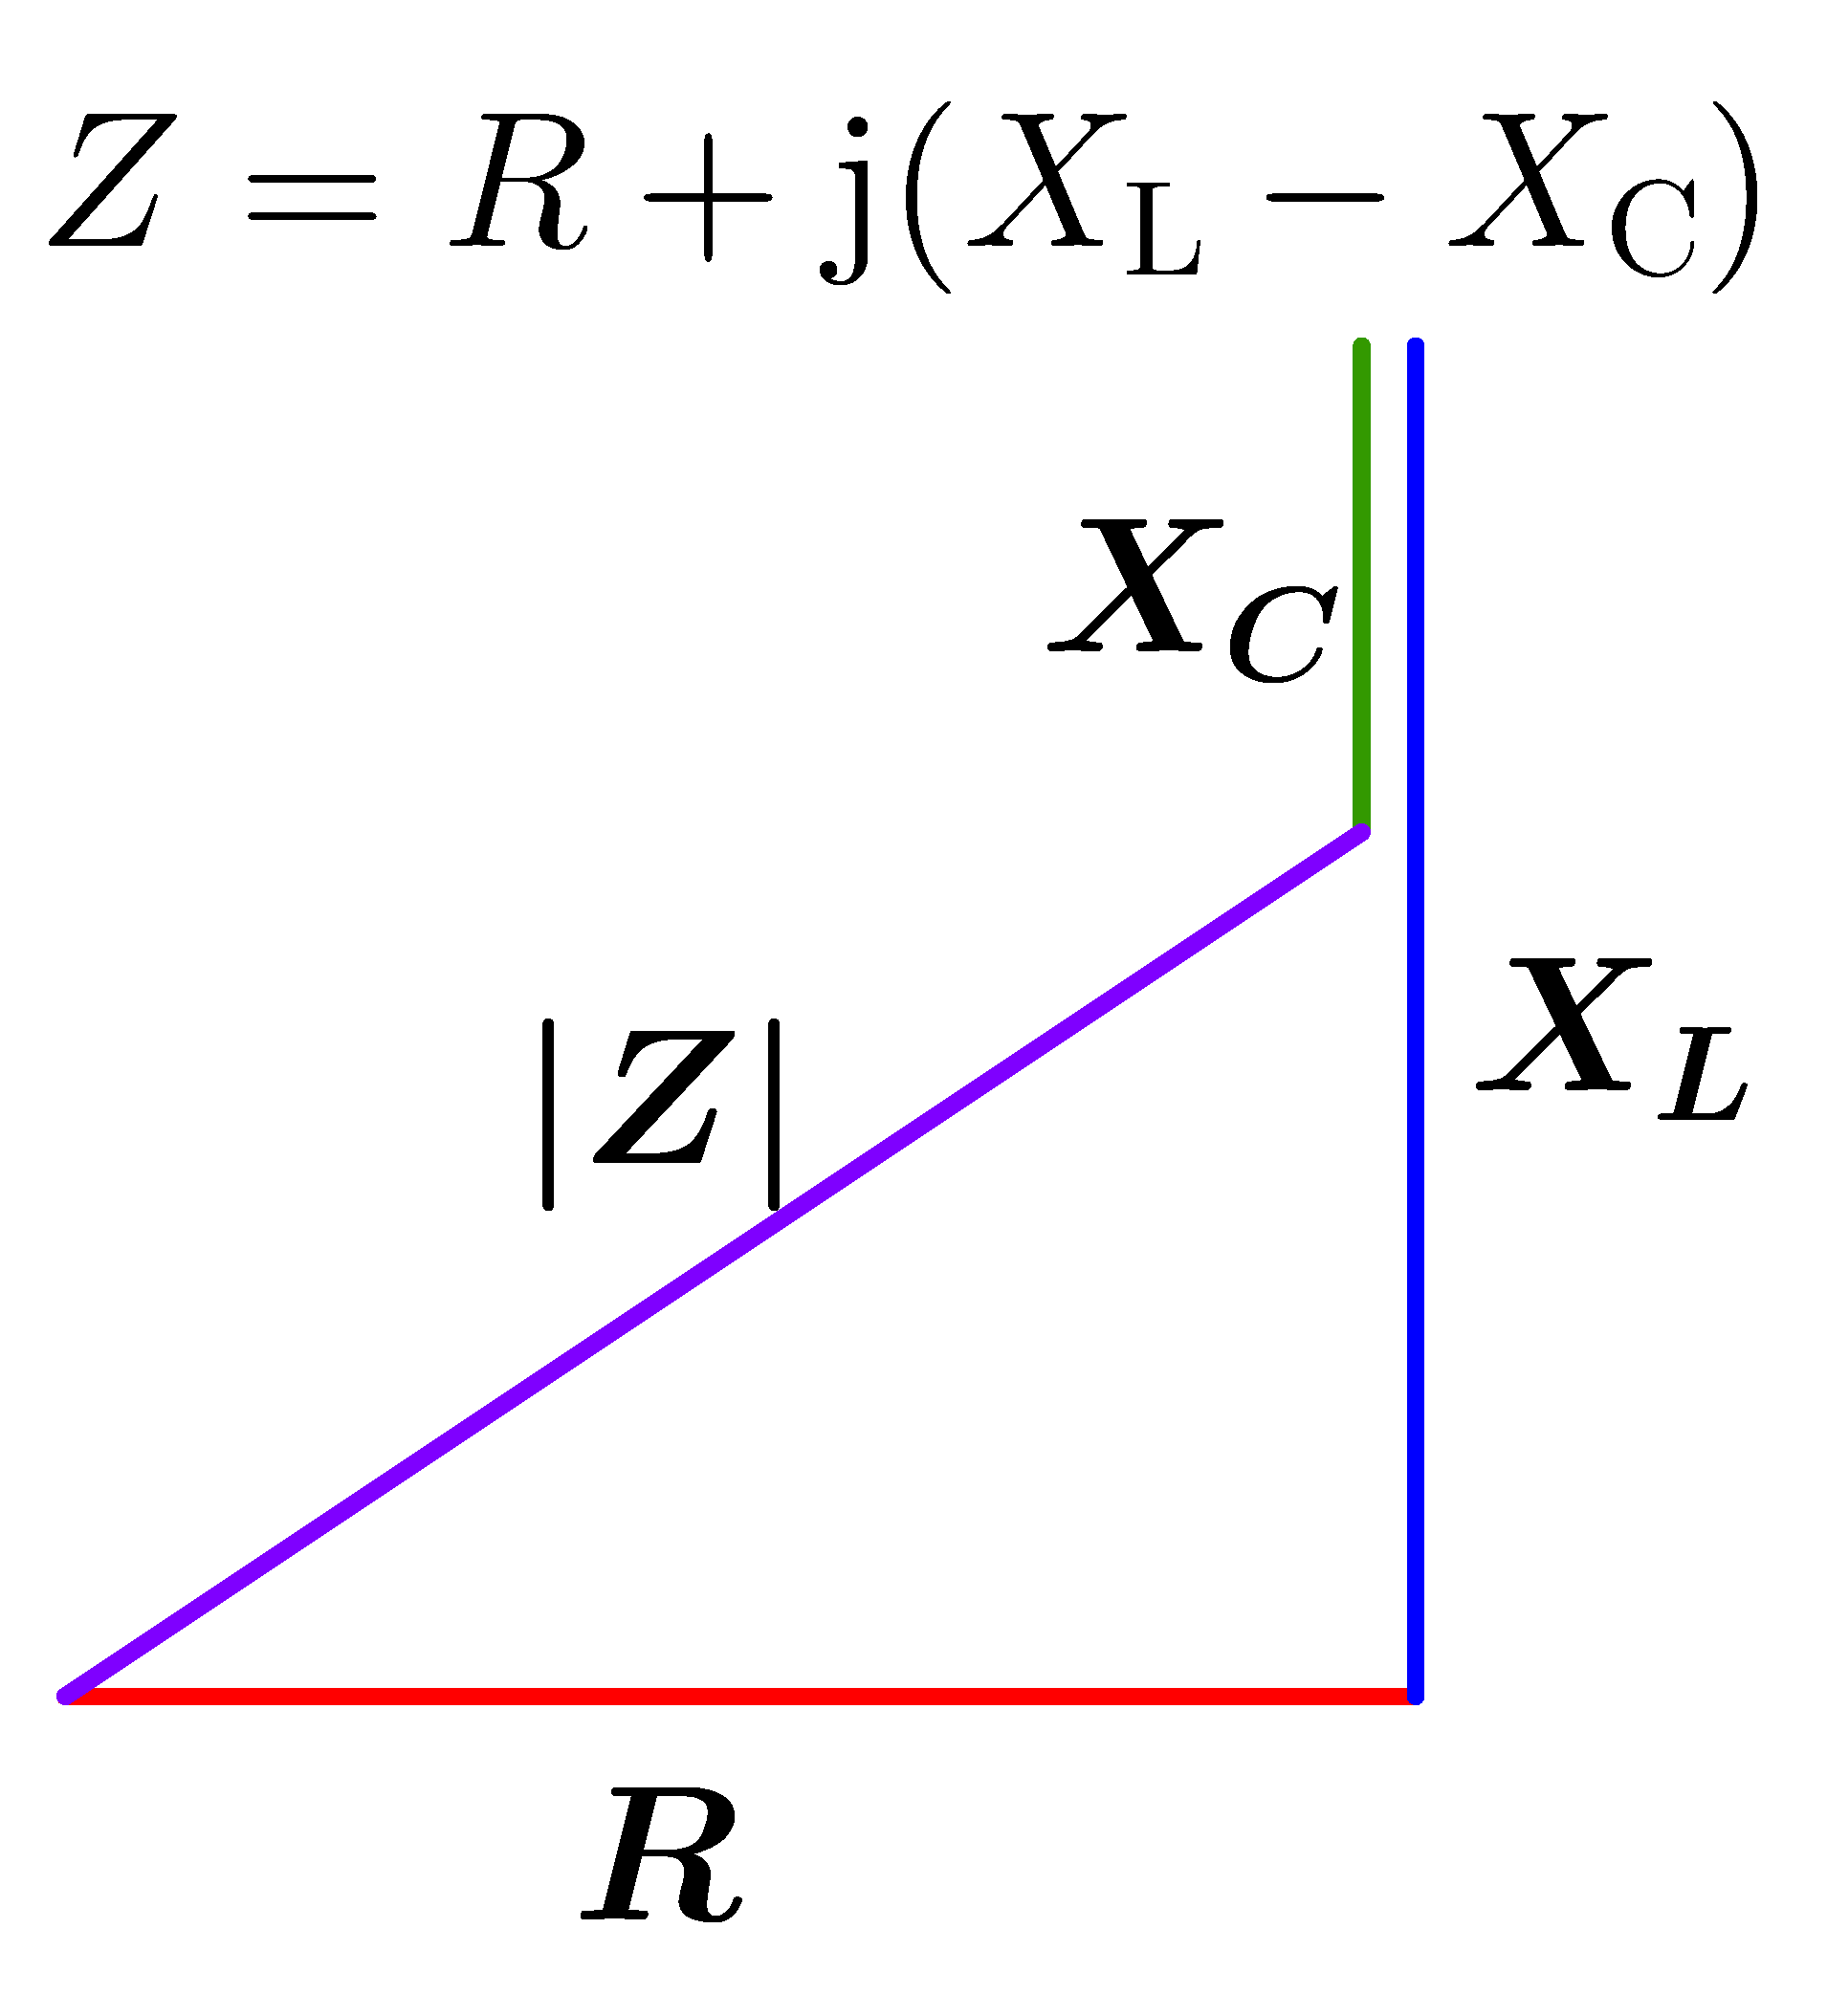
\includegraphics[width=0.95\textwidth]{阻抗三角形.pdf}
        \caption{阻抗三角形}
        \label{fig:阻抗三角形}
    \end{minipage}
    \begin{minipage}{0.3\textwidth}
        \centering
        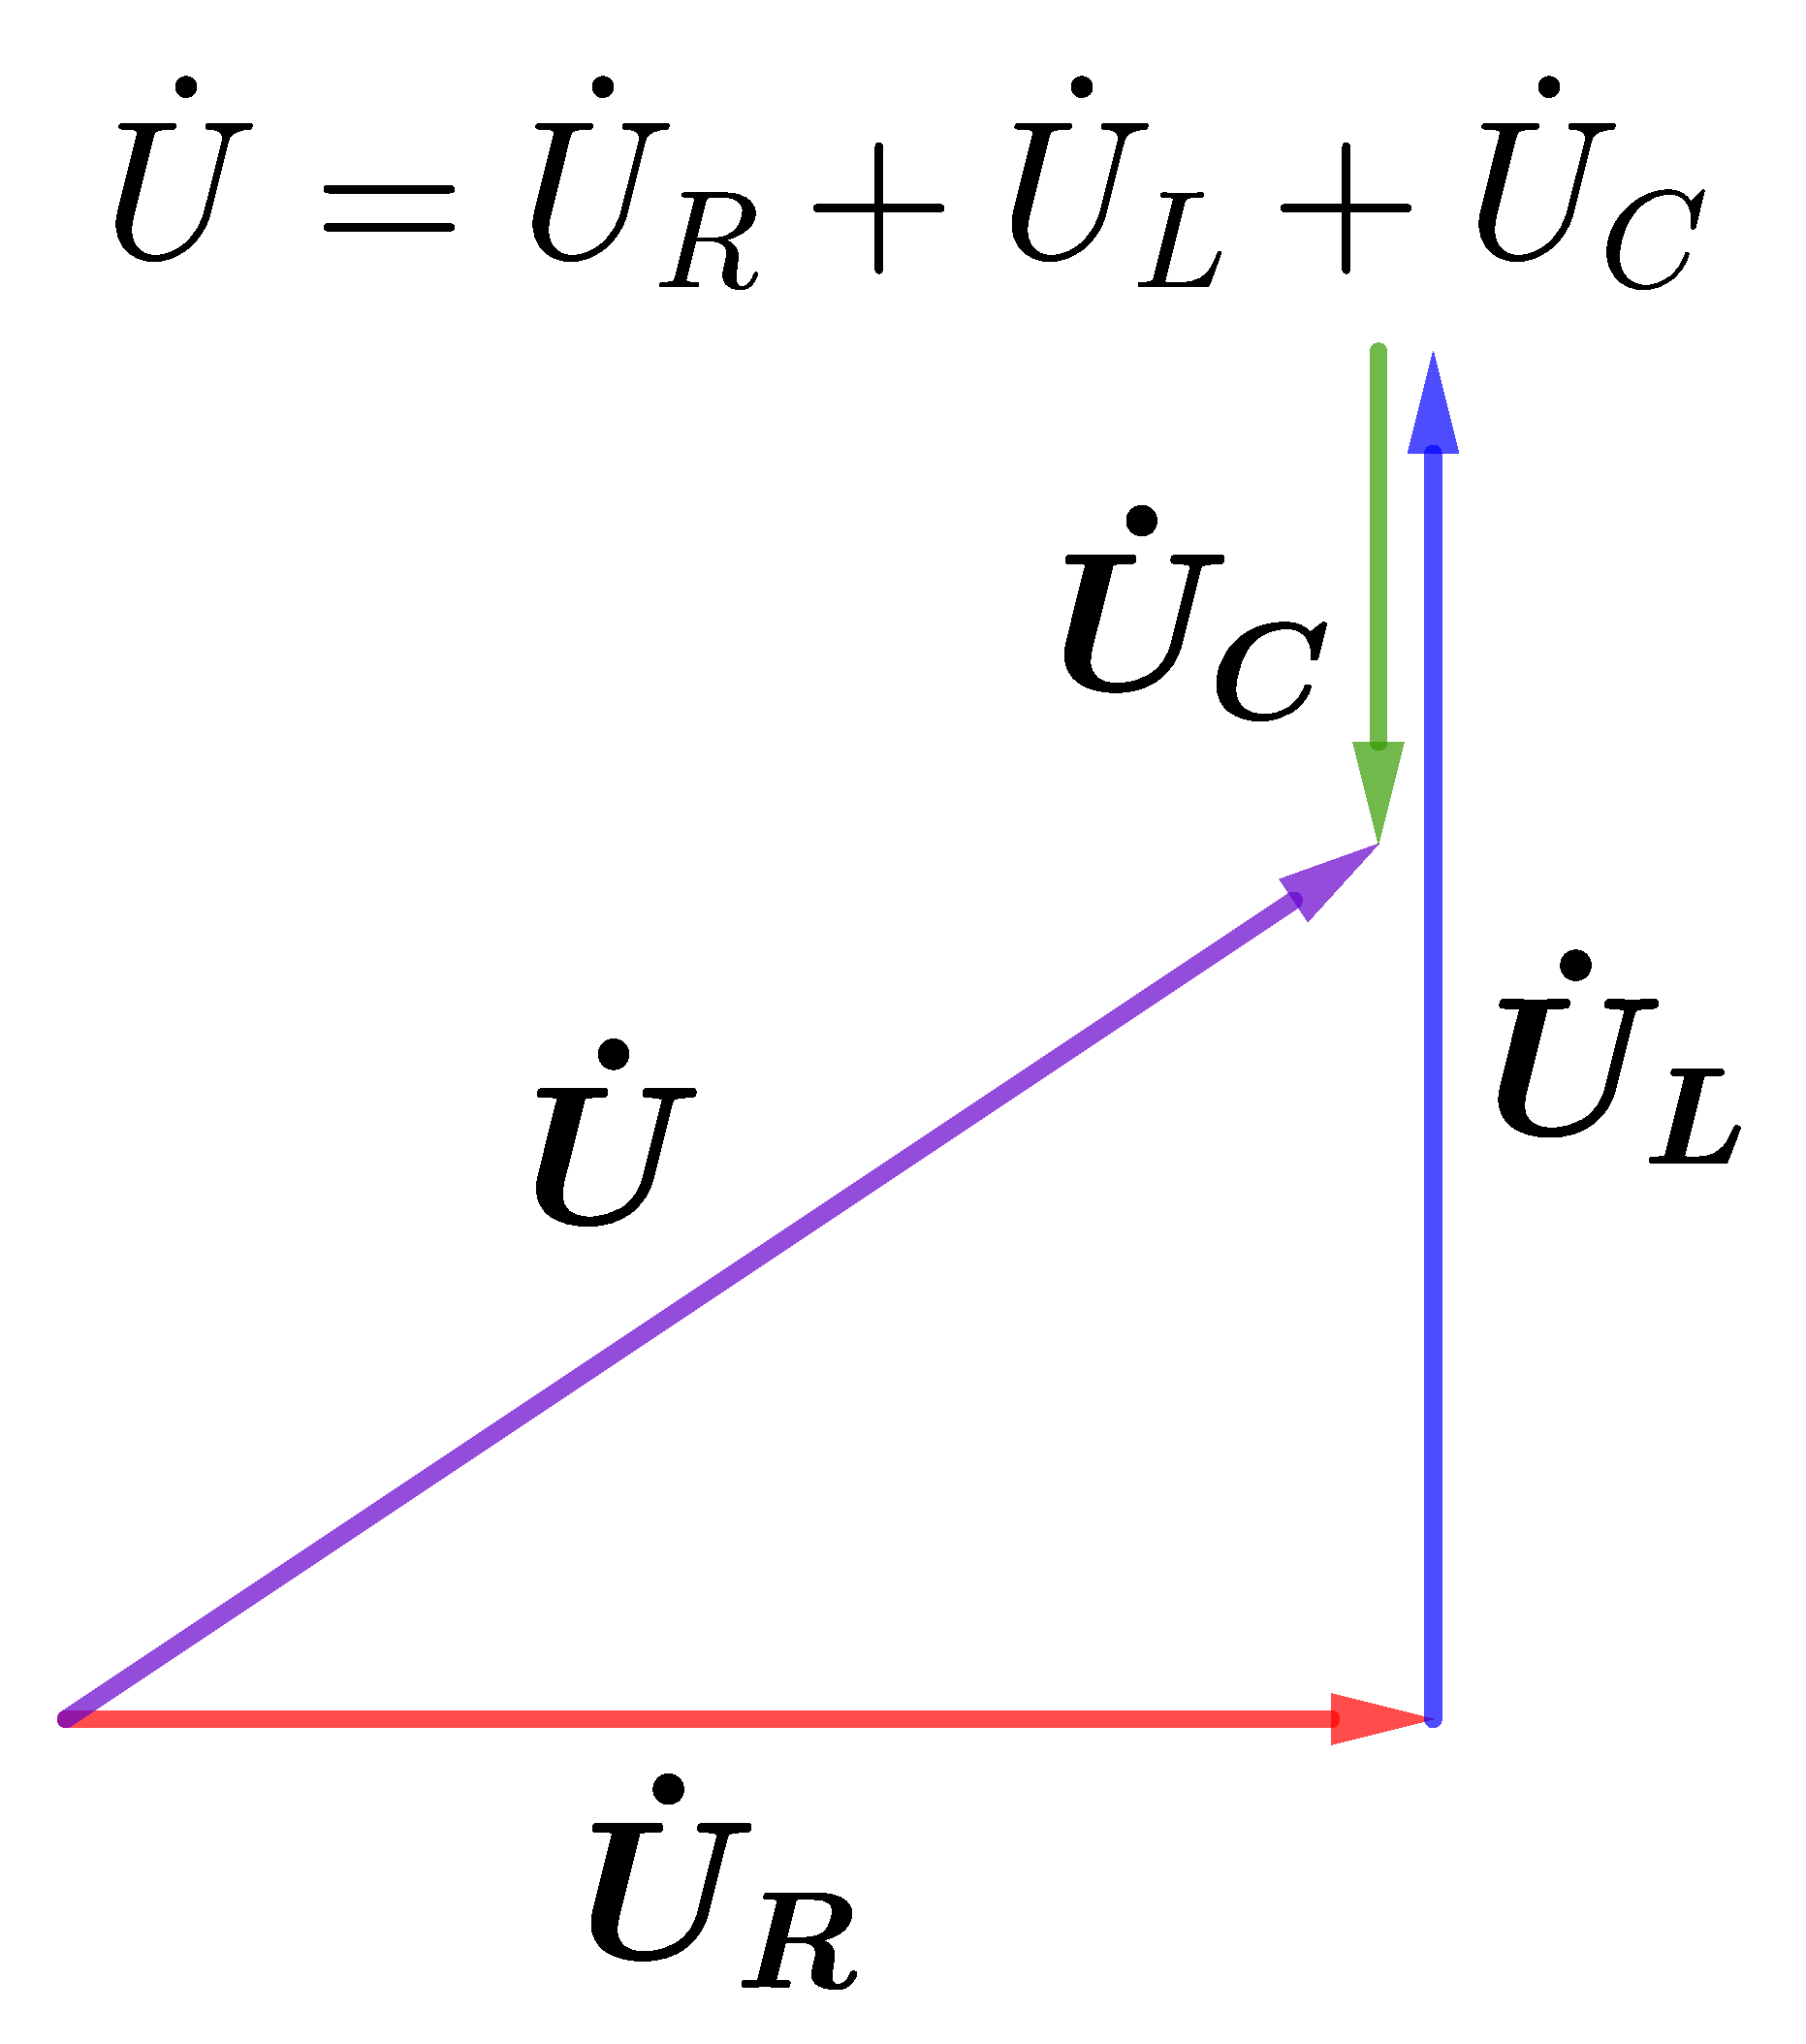
\includegraphics[width=0.95\textwidth]{电压三角形.pdf}
        \caption{电压三角形}
        \label{fig:电压三角形}
    \end{minipage}
    \begin{minipage}{0.3\textwidth}
        \centering
        \includegraphics[width=0.95\textwidth]{功率三角形.pdf}
        \caption{功率三角形}
        \label{fig:功率三角形}
    \end{minipage}
\end{figure}

需要注意的是,只有电压三角形是满足相量关系的三角形,阻抗三角形和功率三角形仅满足数量关系.而它们三者之间还满足
\begin{equation}
    \text{阻抗三角形}\xrightarrow{\text{乘以}I}\text{电压三角形的有效值}\xrightarrow{\text{乘以}I}\text{功率三角形}
\end{equation}


